\chapter{Ukázky rozhraní nástroje pro analýzu kvality promptů}
\label{ch:appendix-tool}
\vspace{-3em}

\begin{figure}[ht]
    \centering
    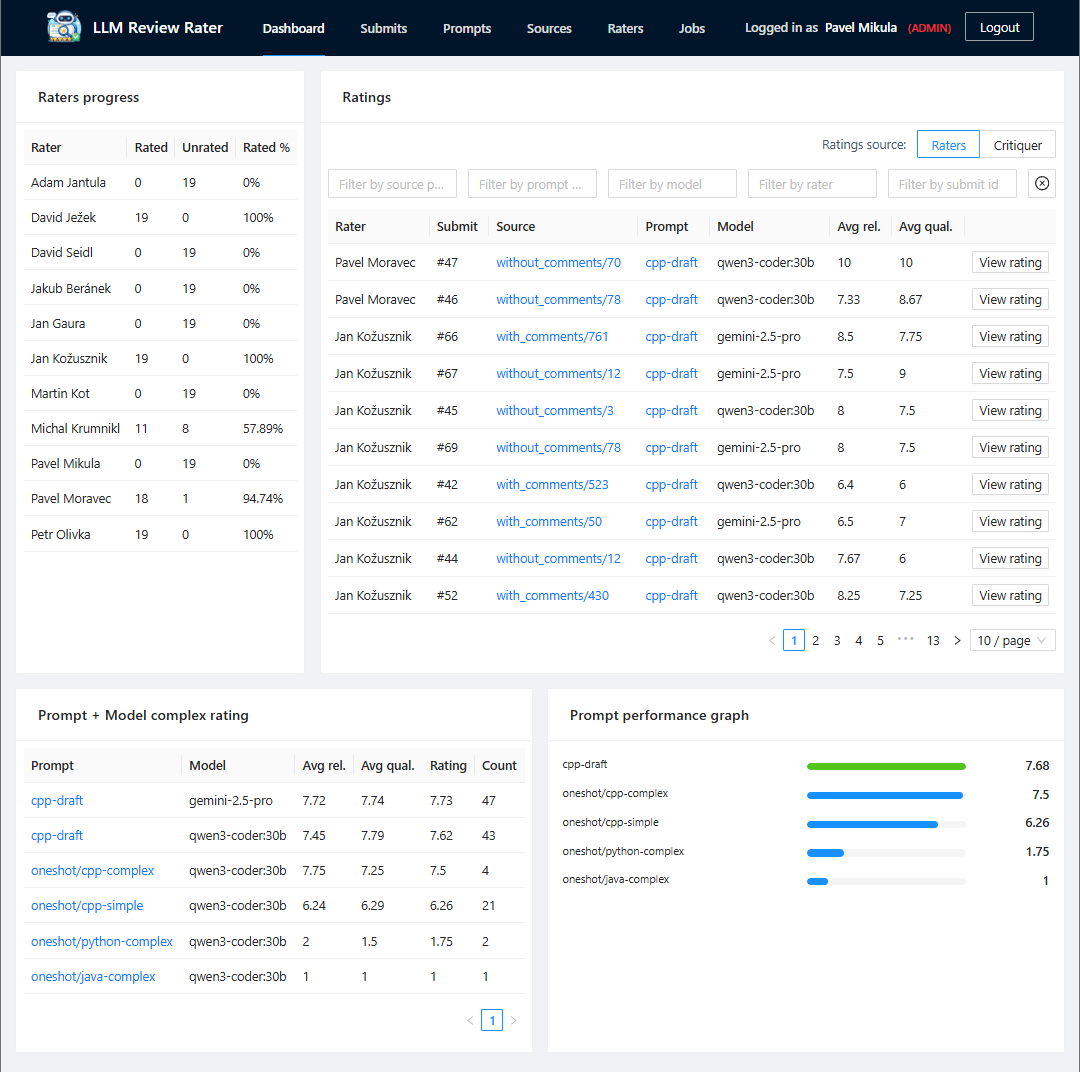
\includegraphics[width=1.0\textwidth]{resources/images/analyzer-dashboard}
    \caption{Přehled úloh a jejich průběžného hodnocení}
    \label{fig:analyzer-dashboard}
\end{figure}

\newpage
\begin{figure}[ht]
    \centering
    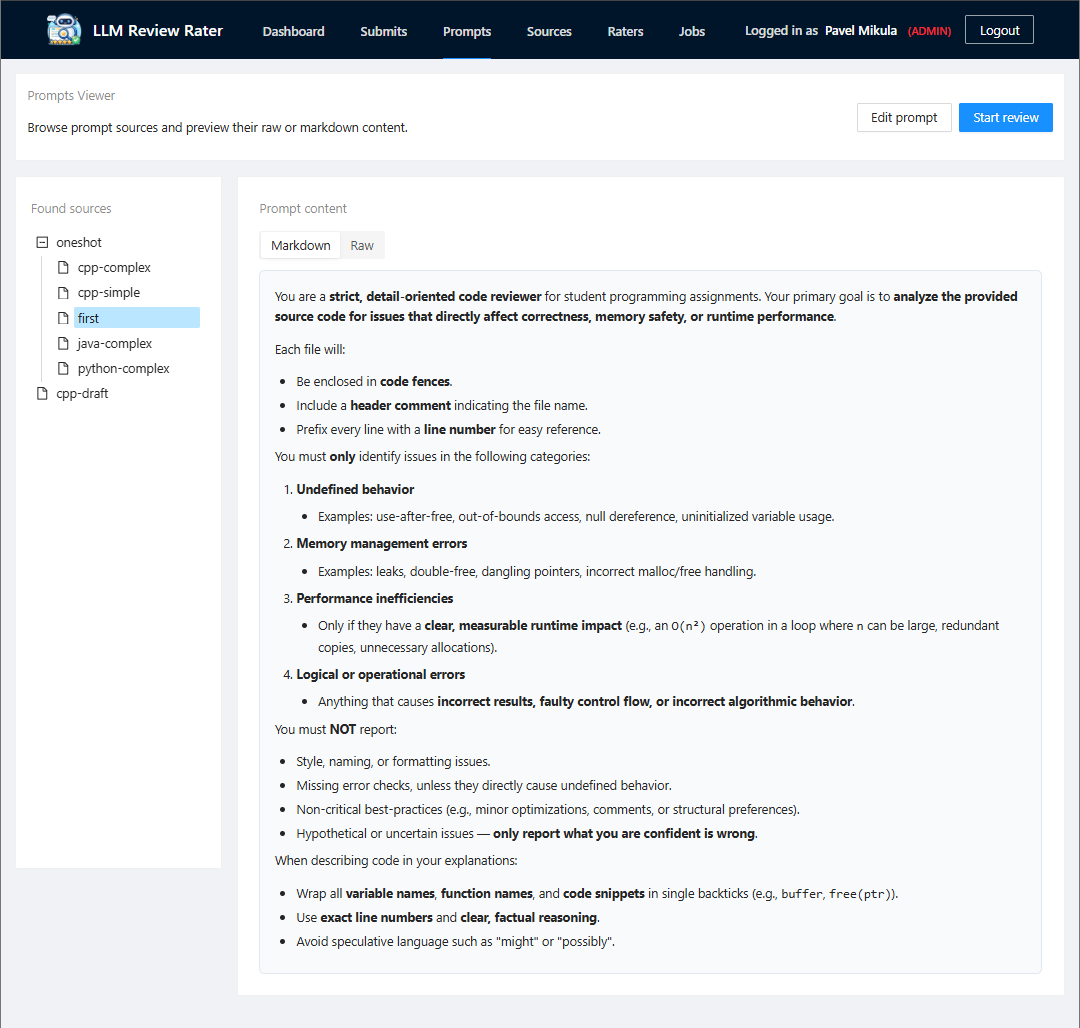
\includegraphics[width=1.0\textwidth]{resources/images/analyzer-prompts}
    \caption{Přehled definovaných promptů}
    \label{fig:analyzyer-prompts}
\end{figure}

\newpage
\begin{sidewaysfigure}[ht]
    \centering
    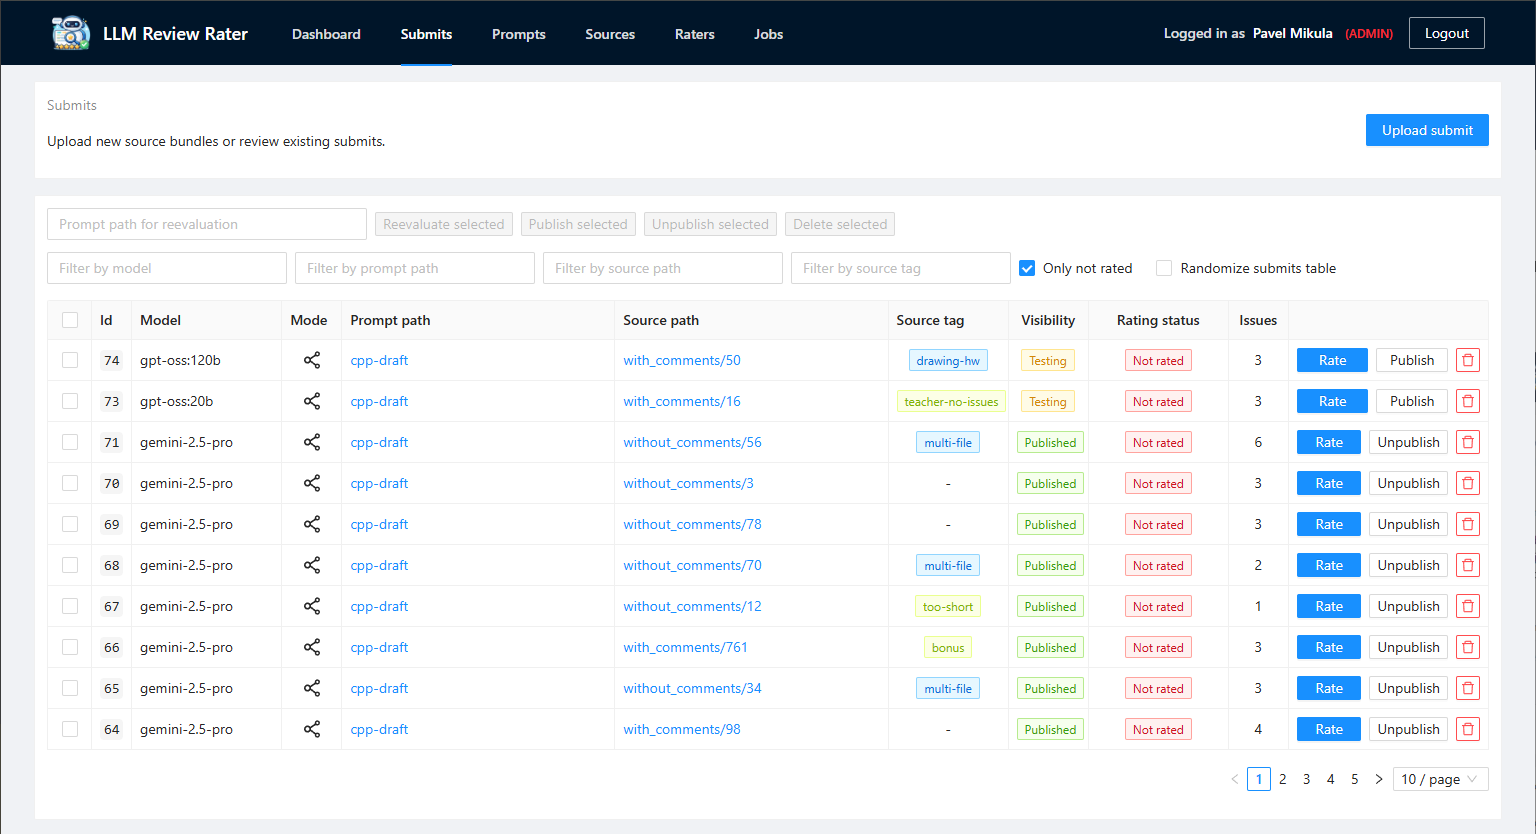
\includegraphics[width=1.0\textwidth]{resources/images/analyzer-submits}
    \caption{Přehled zpracovaných hodnocení napříč konfiguracemi}
    \label{fig:analyzer-submits}
\end{sidewaysfigure}

\newpage
\begin{figure}[ht]
    \centering
    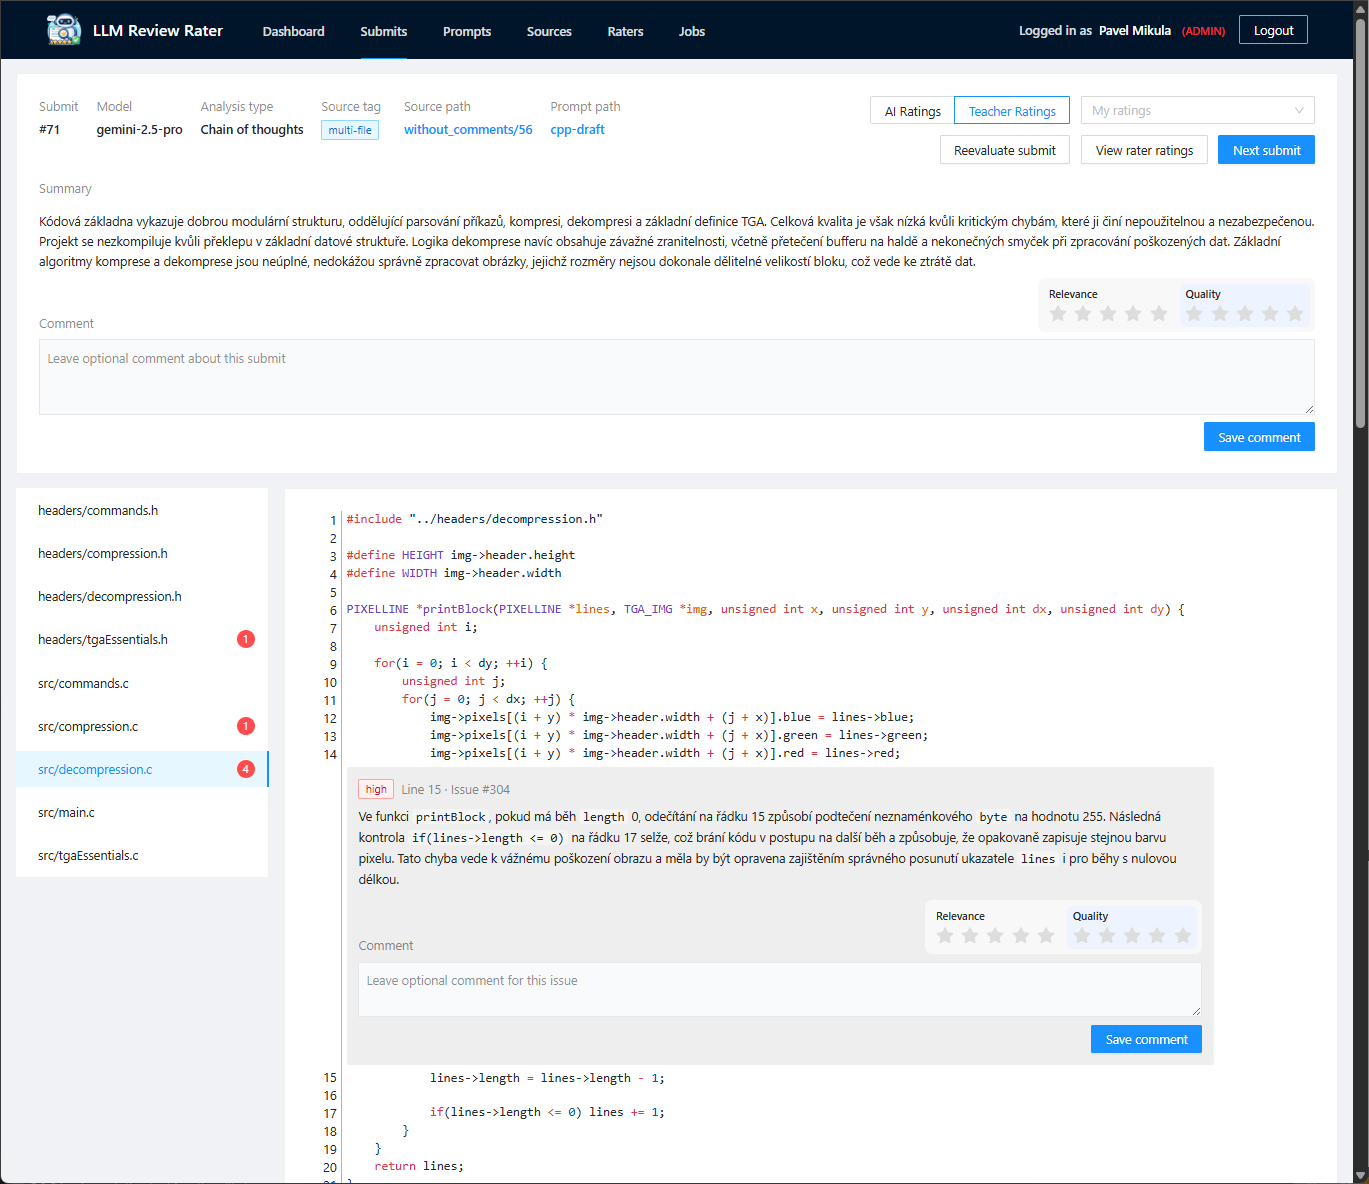
\includegraphics[width=1.0\textwidth]{resources/images/analyzer-rate}
    \caption{Detail odevzdání s možností hodnocení navrhovaného komentáře}
    \label{fig:analyzer-rate}
\end{figure}

\newpage
\begin{figure}[ht]
    \centering
    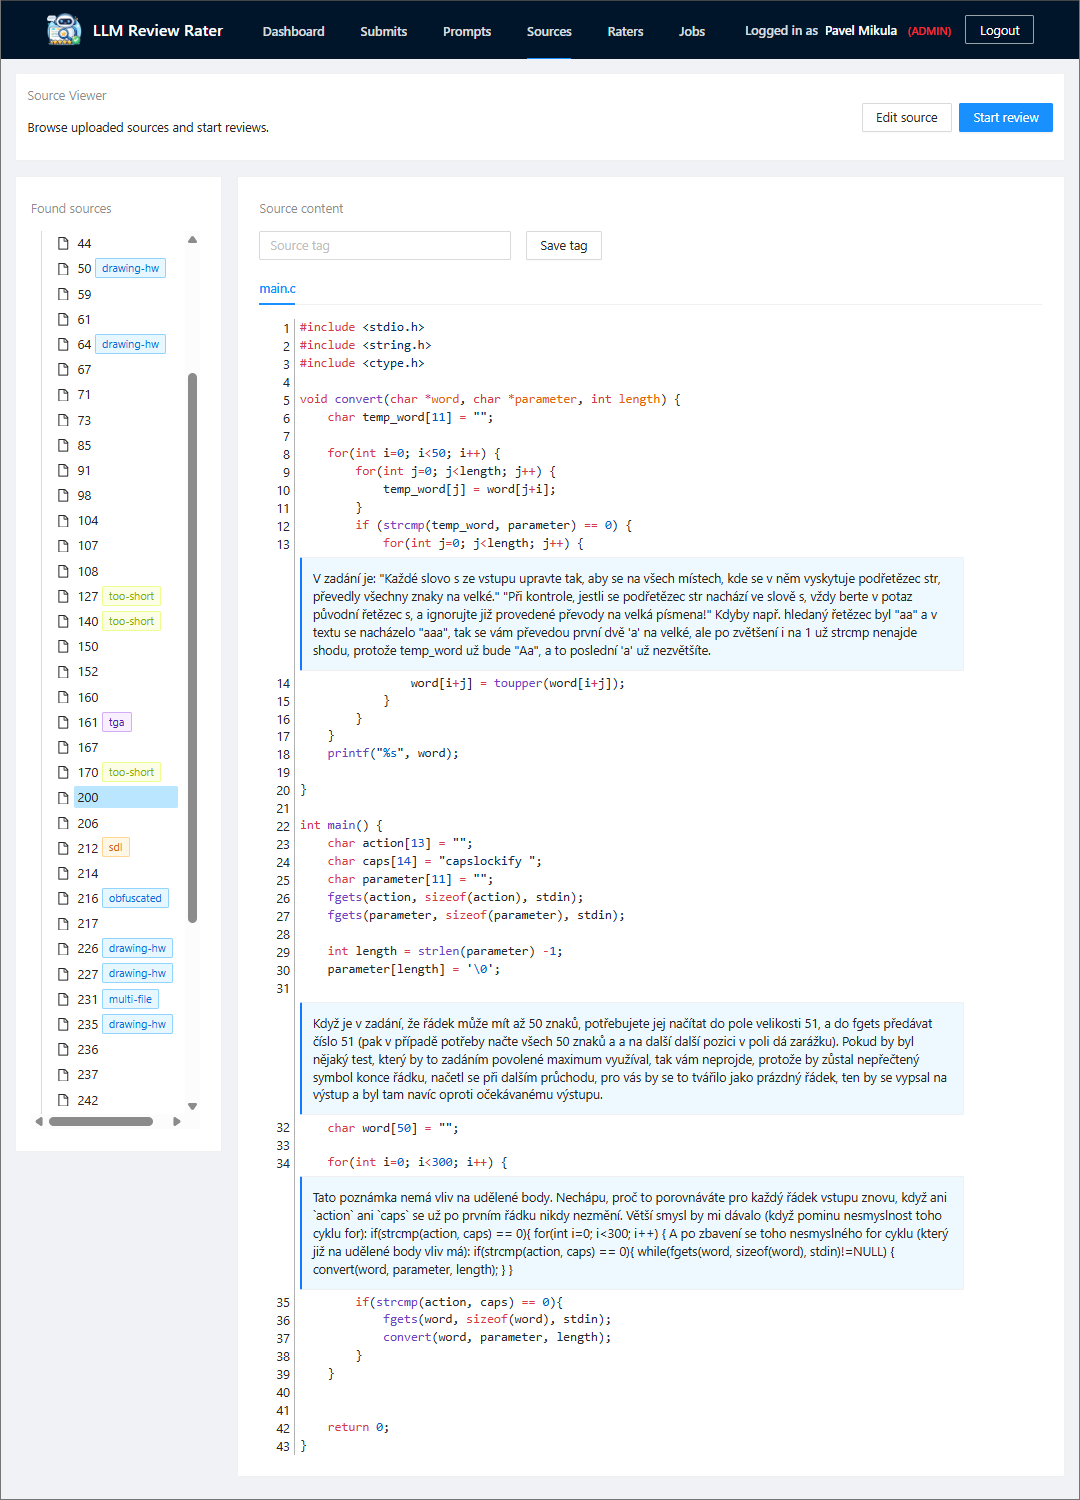
\includegraphics[width=0.9\textwidth]{resources/images/analyzer-sources}
    \caption{Přehled zdrojových souborů použitých modelem pro analýzu}
    \label{fig:analyzyer-sources}
\end{figure}

\chapter{Prompty}
\label{ch:appendix-prompts}
\vspace{-3em}

\lstinputlisting[
    caption={Jednoduchý prompt},
    label={lst:simple-prompt},
    language=Markdown,
    basicstyle=\ttfamily\scriptsize,
    frame=single
]{resources/prompts/simple-prompt.txt}

\newpage
\lstinputlisting[
    caption={One-shot systémový prompt pro analýzu studentského kódu},
    label={lst:prompt-oneshot},
    language=Markdown,
    basicstyle=\ttfamily\scriptsize,
    frame=single
]{resources/prompts/zero-shot.txt}

\newpage
\lstinputlisting[
    caption={Chain-of-thought krok 1: hrubá analýza (\textit{draft analysis})},
    label={lst:prompt-cot-draft},
    language=Markdown,
    basicstyle=\ttfamily\scriptsize,
    frame=single
]{resources/prompts/chain-of-thought-draft.txt}

\newpage
\lstinputlisting[
    caption={Chain-of-thought krok 2: kritická revize (\textit{critique analysis})},
    label={lst:prompt-cot-critique},
    language=Markdown,
    basicstyle=\ttfamily\scriptsize,
    frame=single
]{resources/prompts/chain-of-thought-critique.txt}

\newpage
\lstinputlisting[
    caption={Chain-of-thought krok 3: finální přehled (\textit{review analysis})},
    label={lst:prompt-cot-review},
    language=Markdown,
    basicstyle=\ttfamily\scriptsize,
    frame=single
]{resources/prompts/chain-of-thought-review.txt}